%\renewcommand{\tabularxcolumn}[1]{m{#1}}
%\newcolumntype{Y}{>{\centering\arraybackslash}X}
%\newcolumntype{R}{>{\flushright\arraybackslash}X}


\renewcommand{\thesection}{\arabic{chapter}.\arabic{section}}


\chapter{Investigating the Impact of Uncertainty on Firms with Dynamic Costs : A Case Study of the French Electricity Market}
\label{chap:ch2}
\cleardoublepage

%\doublespacing
In the last chapter, we have given some attention to a methodology that allows us to use functional data for reduced form analysis. In this chapter, we focus on the economic questions that can be asked using such a methodology. Specifically, we focus on an investigation of the effect of uncertainty on the behaviour of electricity producers. 

There exists a consensus that dynamic costs, also referred to as ramping or adjustment costs, are important on the electricity market\footnote{ \cite{anderson2005supply},  \cite{hobbs2001next}, \cite{hortacsu2008understanding}, \cite{reguant2011welfare}, \cite{sewalt2003negative}. }. These are the costs incurred by a producer when production varies. 
The importance of uncertainty for the expectation of dynamic costs is shown in \cite{bergesmartimort2014}. Uncertainty itself on the electricity market has been studied by \cite{wolak2007quantifying}. %, who specifies and captures in a single index the uncertainty that suppliers face on the electricity market. %: (i) the uncertainty from not knowing the aggregate supply function served by all other suppliers and (ii) the uncertainty about the realisation of the market demand. , who specifies and captures in a single index the uncertainty that suppliers face on the electricity market.   
We focus on two sources of uncertainty for traditional electricity suppliers, namely uncertainty about the realisation of the market demand and uncertainty from the inherently unpredictable meteorological situation
%forecasts 
(which affects renewables generation). 
We propose a methodology to measure this uncertainty and its impact on firm strategies on the electricity market. %due to the existence of dynamic costs. %Our methodology allows to address policy questions of high relevance, such as the optimal spatial distribution of renewable production facilities. 

Electricity as a market is very important in and of itself ($\$2$ trillion in worldwide sales in 2010). It is also a crucial input for many industries; power outages induce very large costs to society (\cite{lacommare2004understanding}, \cite{reichl2013power}). 
%The importance of electricity for modern economies is undeniable. Indicators of its importance are the size of its market ($\$2$ trillion in worldwide sales in 2010) and the fact that electricity is an input for many other industries. 
%Market failures, which arise in the form of mis-pricings or network breakdowns, have very large economic costs to society and deserve more attention. 
%The analysis of its markets is highly interesting from an economic perspective. 
The electricity market is, however, quite different from the markets for other commodities in a few respects. First, electricity cannot be efficiently stored. As a consequence, electricity markets are high frequency (prices can update down to 15-min intervals) and firm strategies are purer as they are free of stock management considerations. 

Second and in addition to non-storability, a generation surplus cannot be disposed of freely\footnote{The common assumption of free disposal as made in standard microeconomics is violated.}. Thus, generation of electricity must always be matched with consumption in real time (modulo a small tolerance). This represents a hard constraint on the market\footnote{Mismatches between consumption and generation ultimately result in power outages.} and forces suppliers to be reactive. However, this reactivity is costly as plant operators incur dynamic costs when adjusting production and the larger the adjustment made, the larger the cost. 
Hence, suppliers face a trade-off between cheap generation of electricity and costly reactivity to the demand realisation. Indeed, no single generation technology exists that satisfies both cheap generation and sufficient reactivity to allow production fluctuations at a reasonable price . Existing generation techniques are either cheap and unresponsive, e.g. nuclear plants, or expensive and flexible, e.g. gas turbines. 
 
Interestingly, we also observe negative prices. In France for example, during the weekend of the 15$^\text{th}$ June 2013, the price per MWh dropped to $-200$\EUR{}. This contrasts to the yearly average of approx. $ 45$\EUR{}/MWh and is generally understood as a sign that subsidising consumption temporarily is cheaper for a supplier than shutting down a plant \cite{epexwebsite1}\footnote{``Negative prices are a price signal on the power wholesale market that occurs when a high inflexible power generation meets low demand. Inflexible power sources can’t be shut down and restarted in a quick and cost-efficient manner. Renewables do count in, as they are dependent from external factors (wind, sun)."}.  The increase of the share of renewable generation in the energy mix contributes to the occurrence of negative prices on the market. 
% Renewables generation benefits from a feed-in guarantee on the electricity grid. 
The intermittency of renewables causes large residual demand shocks \cite{epexwebsite1}. The unreliability of renewable generation also means that more flexible plants (i.e. plants with lower dynamic costs) are required to provide rapid responses to fluctuations in production from renewables \cite{ren2013renewables}. 

Furthermore, uncertainty arises from the fact that renewable production is a local and dispersed production, but feeds into a national market with a single price. When meteorological conditions change, the geographic production profile also changes. This further complicates the predictability of renewables generation and contributes to the uncertainty that electricity producers face when playing %bidding 
on the electricity %EPEX Spot 
market \cite{meibom2009operational}.

This paper explores the effect that the absolute level of uncertainty about residual demand has on players' strategies on the electricity market. In the light of the existence of dynamic costs, which are inherent to the production technologies,  uncertainty is costly to suppliers \cite{bergesmartimort2014}. Thus when faced with uncertainty, we expect that electricity producers smooth production volume over time in order to minimise dynamic costs. In a single market interaction with a symmetric oligopoly and linear demand functions this translates to playing a steeper supply function when uncertainty is high. The detailed intuition behind the predictions tested is given in section \ref{intropredict}. 

\label{introresults}
We show that uncertainty does impact supplier strategies. However, this prediction and result only apply locally to the central, flat and linear part of the supply bid function. Towards the high and low volume extremities of the bid functions when capacity constraints start to matter, bid functions become vertical and the effect of uncertainty vanishes. Furthermore, we observe results that indicate that demand-side bidding is also impacted by uncertainty.  
%However the prediction tested is only partially validated by the data, in that only part of the curves are indeed getting steeper as uncertainty increases whereas others get less steep. We discuss how and why those discrepancies might arise at the end of the paper.  

%In the light of the existence of dynamic costs, which are inherent to the production technologies,  uncertainty is costly to suppliers \cite{bergesmartimort2014}. 
%The industry set-up allows suppliers to trade the uncertainty on three different markets that differ the lead time up to delivery *** OR 
%The converse holds: acquisition of information about expected residual demand is valuable. 
%The industry set-up allows the incorporation of new information about expected demand by its segmentation into three markets that differ by the lead time up to delivery: 
%a longterm bilateral contracting market, a one-day ahead market and an intraday balancing market for last-minute adjustments. 

We focus on the French one-day ahead market, EPEX Spot. This market is a divisible goods auction and 
particularly suited for our analysis as we observe data on the full aggregate bid functions for both supply and demand.  We introduce the market's auction format and rules in section \ref{epexall}.
%***** WE CHOOSE MARKET BECAUSE OF DATA AVAILABILITY NOT BECAUSE OF SPECIFIC PLACE IN INDUSTRY -> CAUSALITY NOT 
%we explore the link between uncertainty and dynamic costs. Theoretical models imply that uncertainty about the market outcome impact player's strategies on the market \cite{bergesmartimort2014}. More specifically, this paper aims to better understand the shape of aggregate bid functions on the EPEX Spot market and tests the impact of the absolute level of uncertainty  on the submitted bid functions of suppliers. In the presence of dynamic costs, we expect that electricity producers smooth production volume over time in order to minimise these dynamic costs. In a single auction this translates to bidding a steeper supply function when uncertainty is high. The detailed intuition behind the predictions tested is given in section \ref{intropredict}. 
The dataset and its sources are presented in section~\ref{datasection}.
We develop our identification methodology in section \ref{newapproach}. Our empirical strategy relies on the non-parametric, comparable point selection technique presented in chapter \ref{pschapter}. 
We reuse the selected points of the previous chapter for our analysis here. 
We present and interpret the results in section \ref{resultsplusinterpret}. 
%In section XXX, we focus on welfare analyses.**** TO DO : We first apply the model to quantify the effect of uncertainty in terms of price differentials on the market and then address the social cost, which could be avoided if geographic plant location was not decided on by individual investors, but by a social planner, who minimised uncertainty of renewables production. 
Finally, we discuss some overarching points in section \ref{discussgeneral} and conclude in section~\ref{conclusion}.




\subsection{Literature review and contribution}
\label{litrev}

There exists a literature on supply function equilibria initiated by \cite{KM}. 
In traditional models, firms choose between quantities (Cournot) or prices (Bertrand) as their strategic quantities. In the intermediate case, firms choose a relationship between quantities and prices, namely a supply function. This is the focus of the supply function equilibrium models.
%In this literature, firms do not have to choose between prices or quantities as a strategic variable, but submit a supply function which matches the quantity supplied by the firm to the price of the market. %, which endogenously determined by the aggregate supply and demand. 
A key ingredient of these models is uncertainty.

Supply function equilibrium models are very relevant for the analysis of electricity markets, since many electricity market designs allow firms to submit a price-volume function rather than a specific price or quantity. \cite{Newgreen}, \cite{newbery1998competition} and \cite{bolle1992supply} have used these models to analyse competition on the electricity markets. 
These papers have contributed to a broader investigation of the competition on the electricity markets, which has also been looked at from empirical perspectives \cite{wolfram1998strategic, borensteinetal2002marketineffs}.
While those initial papers have focussed on the supply function equilibria of the market, they have abstracted from some technological specificities for the sake for simplification. 

One such aspect that we are interested in and that has been the subject of research in recent years is the importance of dynamic costs for electricity production. 
% First paper:
\cite{bergesmartimort2014} extend \cite{KM} to derive predictions on firms facing dynamic costs in a supply function oligopoly under uncertainty. 
They find that when varying production is costly, suppliers take these costs into consideration by submitting steeper functions when facing more uncertainty, in order to limit the range of variation in production.
\cite{reguant2011welfare} develops a model and an empirical strategy to measure dynamic costs on the Spanish one-day-ahead electricity market. She finds that ``complex bids", which allow firms to minimise dynamic costs by linking production in one time period to production in a subsequent time period, reduce the volatility and the level of prices on the market.  Her work is also unique in terms of data availability. By using individual bid functions she is able to produce estimates of start-up and ramping costs per production technology. 
In order to quantify dynamic costs on the Australian electricity market, \cite{wolak2007quantifying} derives a methodology to recover estimates of the parameters of parametric cost functions at the level of the production unit. His identification is based on the assumption that each profit maximising supplier knows the distribution of shocks on the demand function when playing on the market. Uncertainty is thus an explicit ingredient of his paper and he captures two sources of uncertainty in a single index: (i) the uncertainty from not knowing the aggregate supply function served by all other suppliers and (ii) the uncertainty about the realisation of the market demand.  The recovered cost functions quantify the cost of varying output. Forward contracts are useful to avoid output variations. By comparing the observed  level of forward contracting (assumed to be the profit maximising choice for production variation) with the theoretical minimum cost production pattern, he %cannot reject the hypothesis that ramping costs are important for suppliers. 
does not find support for ramping costs.

We contribute to this literature by providing an empirical analysis of the French electricity market.
Specifically, we look at the impact of uncertainty on supplier strategies and take this as evidence that dynamic costs matter. 
 Our approach to separate out the uncertainty from market demand expectations and predictability of renewables generation is novel. Both proxies for uncertainty used are new, uncertainty from market demand is inferred from the prediction errors that firms make in a demand estimation and uncertainty from renewable production is computed in a bottom-up approach from local weather forecasts.
Instead of opting for a time series regression, we understand all hourly auctions as a cross-sectional dataset and control for the time of the day by using continuous transition variables for daytime periods. Similarly, we control for seasonality using continuous variables rather than dummies.  Thereby, %we circumvent the problem of dummies in our regressions, which are black boxes for the interpretation.
we are able to leverage our dataset and increase the sample size for each of our regressions and improve the precision of our estimates. 


%maybe 4. (authors of Operational costs induced by fluctuating wind power production in Germany and Scandinavia) give the link from production intermittency of renewables to operational costs for the market. In particular, they separate out the operational costs due to predictatbility and variability of renewables generatio. 

%
%\subsection{Larger research question - link to electricity storage and demand response policies}
%This paper feeds into a larger research project on how a government should allocate resources between developing renewable's generation and alternative policies, such as incentivising research on electricity storage or the pushing of demand response policies. 
%
%Electricity storage refers to techniques to defer consumption of electricity to a later point in time\footnote{** Say example, say problems: Power-to-gas, too expensive on large scale}. 
%Demand response measures allow to reduce electricity consumption at peak times, e.g. by deferring or deleting consumption on the grid\footnote{** say example and problems, "effacement energetique, pas repandu en europe, existe aux US, probleme contraignant.}. 

Furthermore, our work contributes to the empirical literature testing strategic behaviour of market participants. 
 Generally, these studies focus on point-wise analyses for reasons of data availability. Not only does this cause endogeneity problems when the data used is equilibrium data, but also the analysis is restricted to an understanding of the usually observed outcomes of the market. 
In our setting, we benefit from an interesting dataset in which we observe full aggregate bid functions of players. The functions describe the players' behaviour both in the region where the equilibrium is likely to occur as well as in regions that  rarely have an impact on the equilibrium outcome. As such, they provide a much fuller description of the firms' strategies. 
The additional information contained in the full aggregate bid functions has been used extensively in theoretical work (notably in the supply function equilibria literature mentioned above). 
However, few papers exploit these full bid functions empirically. 
%
%This work is also related to another strand of the literature concerned with the functional analysis of data in an economic context. From a theoretical perspective, we many theoretical papers have derived predictions on the supply or demand functions\footnote{CITE SOME LINEAR EXAMPLES.}. However, often subject to strong simplifications such as using linear functions. In the domain of non-linear functions, we observe the work by SOME EXAMPLES. 
%
%From an empirical perspective, functional analyses remain the exception, arguably for reasons of data availability.
For the government bond market, \cite{pw2002etude} and \cite{ozcan2004logistic} use a parametric approach to this functional data for a description of the variation of bid functions with respect to exogenous factors and an investigation of the revenue superiority of the uniform or discriminatory multi-unit auction mechanism, respectively. On the electricity market,  \cite{wolfram1999measuring} leaves the analysis of equilibrium data to investigate duopoly power of firms on the UK day-ahead spot market. Instead, she uses information from the whole aggregate supply function to investigate the impact of price caps for electricity producers. Using an analysis conditioned on 25 different demand levels, she shows that the introduction of price caps resulted in a counter-clockwise rotation of the aggregate supply function. She relates these results to produce a lower bound on the extent to which firms can increase their prices above marginal costs when regulatory pressure makes it advantageous to do so. Thereby, she contributes  empirical evidence for the distorting effects of price caps. 

Our work adds to this empirical literature using the information contained in the full bid functions 
by developing a non-parametric approach which allows to condition our analyses on multiple, representative points of the bid functions. The statistical ingredients rely on \cite{ramsaysilverman2005functional} and are detailed in chapter \ref{pschapter}.
Thereby we are able to leverage our dataset, increase the sample size in individual regressions as well as obtain a fuller picture of the effects of exogenous variables on the behaviour of electricity producing firms. We emphasize that out approach allows to overcome structural restrictions underlying previous parametric approaches, e.g. the symmetry of the logistic function used in \cite{pw2002etude}.

%this literature by  on functional analyses, specifically to that on the electricity market. By conditioning our analysis on different points of the market bid functions, we are able to investigate non-linear effects of exogenous factors on the shape of the bid functions.  While functional analysis have been used in the past, our non-parametric, point-specific approach is novel in the economics literature. Our approach  


\subsection{Theoretical prediction}
\label{intropredict}

%%%%%%%%%%%%%%%%%%%%%%%%%%%%%%%%%%%%%%%%
%%%%%%%%%%%%%%%%%%%%%%%%%%%%%%%%%%%%%%%%
%*** ADD OBJ FUNCTIONS AND QUick DERIVATION TO SUPPORT INTUITION
%%%%%%%%%%%%%%%%%%%%%%%%%%%%%%%%%%%%%%%%
%%%%%%%%%%%%%%%%%%%%%%%%%%%%%%%%%%%%%%%%

We test the impact of uncertainty of supplier strategies by testing the prediction that suppliers bid steeper supply bid functions when faced with a larger uncertainty concerning the outcome of the (residual) demand realisation.
%More specifically, in this paper we aim to better understand the shape of aggregate bid functions on the EPEX Spot market and test the impact of the absolute level of uncertainty on the suppliers submitted bid functions. 

In a discontinuous setting, where the supplier produces volume $Q_H$ of electricity in hour $H$, we assume that he faces a cost function $C_i(.)$ for each production plant $i$. This cost function depends on both marginal costs of production as well as the dynamic costs for changing production rapidly: $C_i \bigl( (Q_H), (Q_H - Q_{H-1})^2 \bigr)$. The larger the variation in production between hours, the larger the dynamic costs. 
Even when the expected residual demand is constant, there are still fluctuations in the production due to possible shocks to the residual demand. The larger the shocks, the larger the change in production and thus the larger the dynamic costs. 
%Given a constant expected residual demand, unpredictable shocks on the demand function induce these dynamic costs. 
Consequently, increased uncertainty (as represented by shocks on the demand function) translates into increased expected dynamic costs. We assume that the profit maximising supplier knows the distribution of shocks on the demand function when choosing his supply function.  In order to minimise these costs, the producer can choose a steeper supply function when uncertainty is high. We want to test this prediction. 

%The intuition behind the predictions tested in this paper is illustrated in figure \ref{predictslope} using a stylised case. 
We illustrate the intuition behind this prediction using a stylised case in figure \ref{predictslope}. The graphs depict a situation in which a single, risk-neutral supplier bids a supply function to supply electricity in the hours 9 and 10 of the next day. For both hours, the supplier faces a constant expected residual demand function represented by $E(D)$. In a static optimisation problem, the supplier would bid a supply function $S_0$ in both auctions. 

\begin{figure}[!ht]
\begin{center} \makebox[\textwidth]{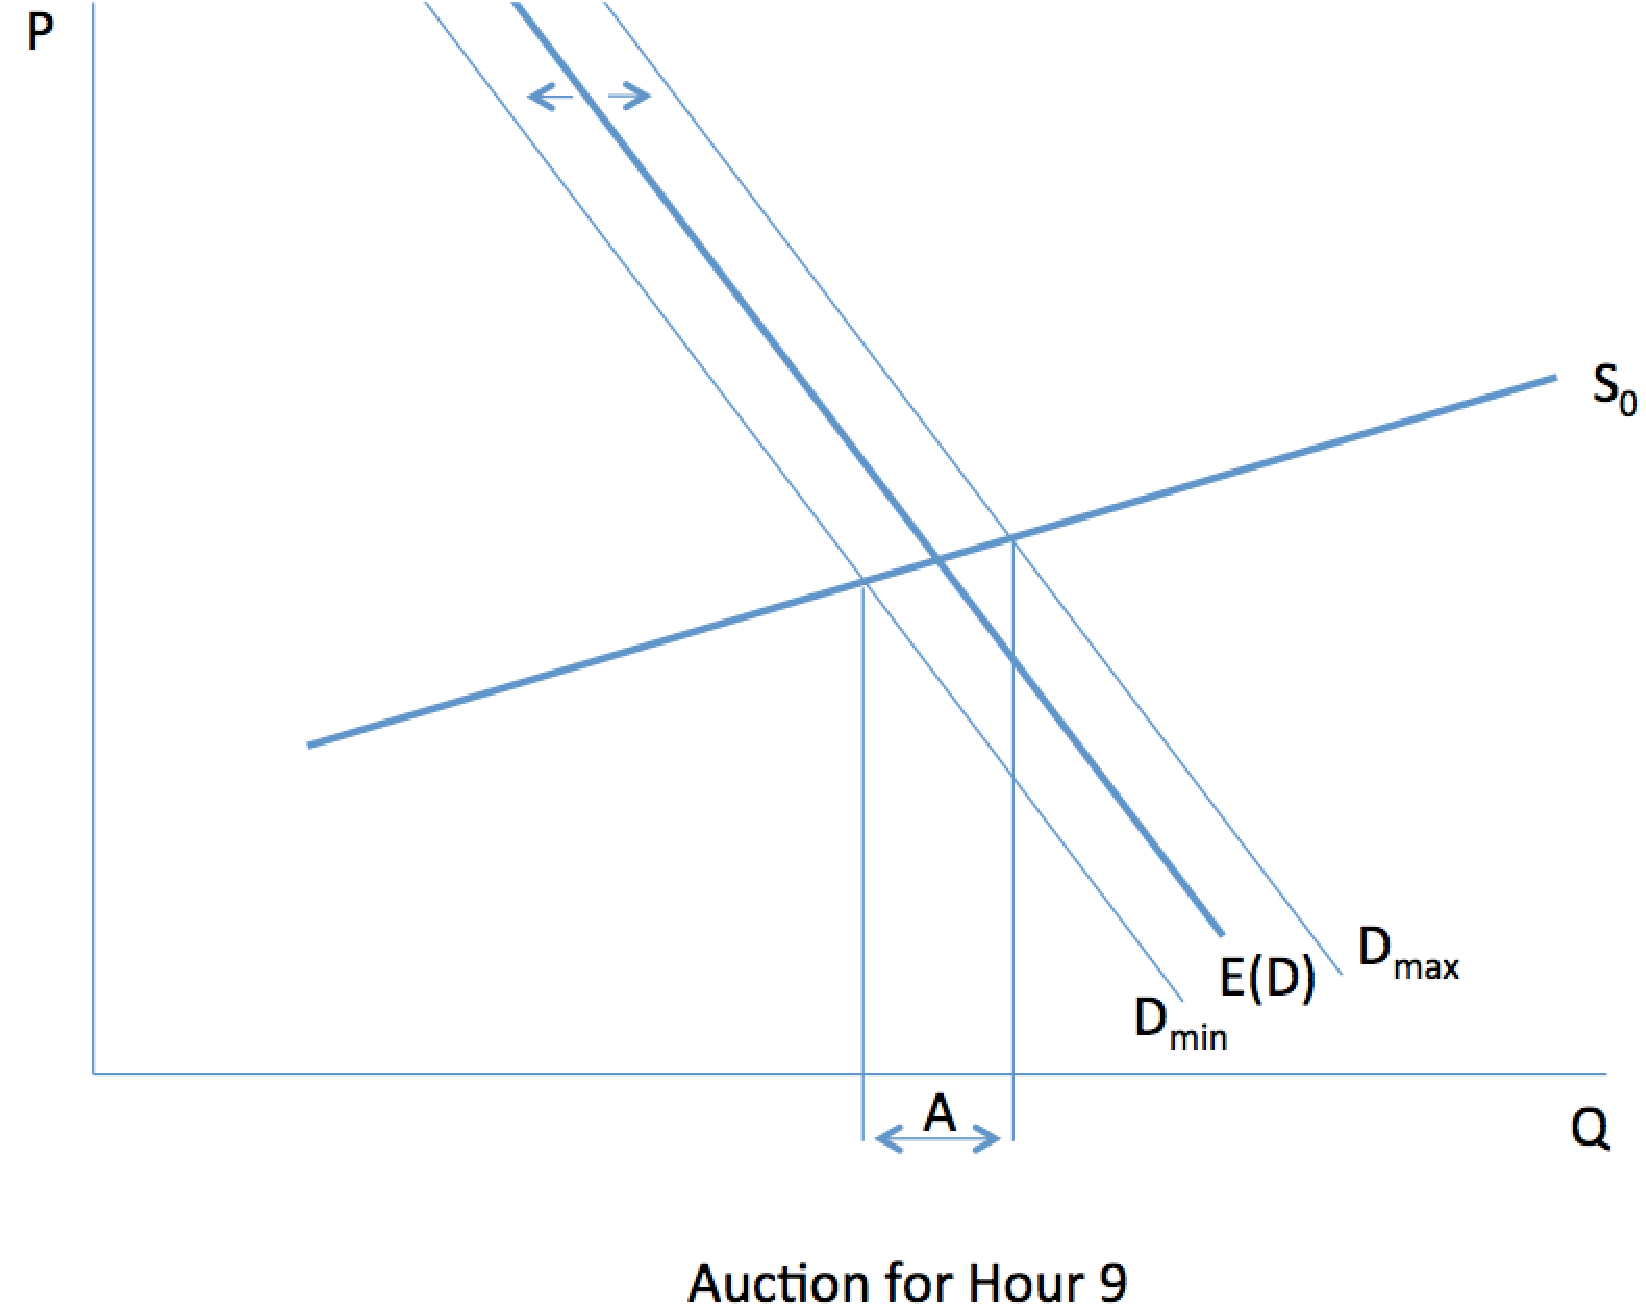
\includegraphics[height=50mm]{figch2/Shot35.pdf} \hspace{0.03cm} 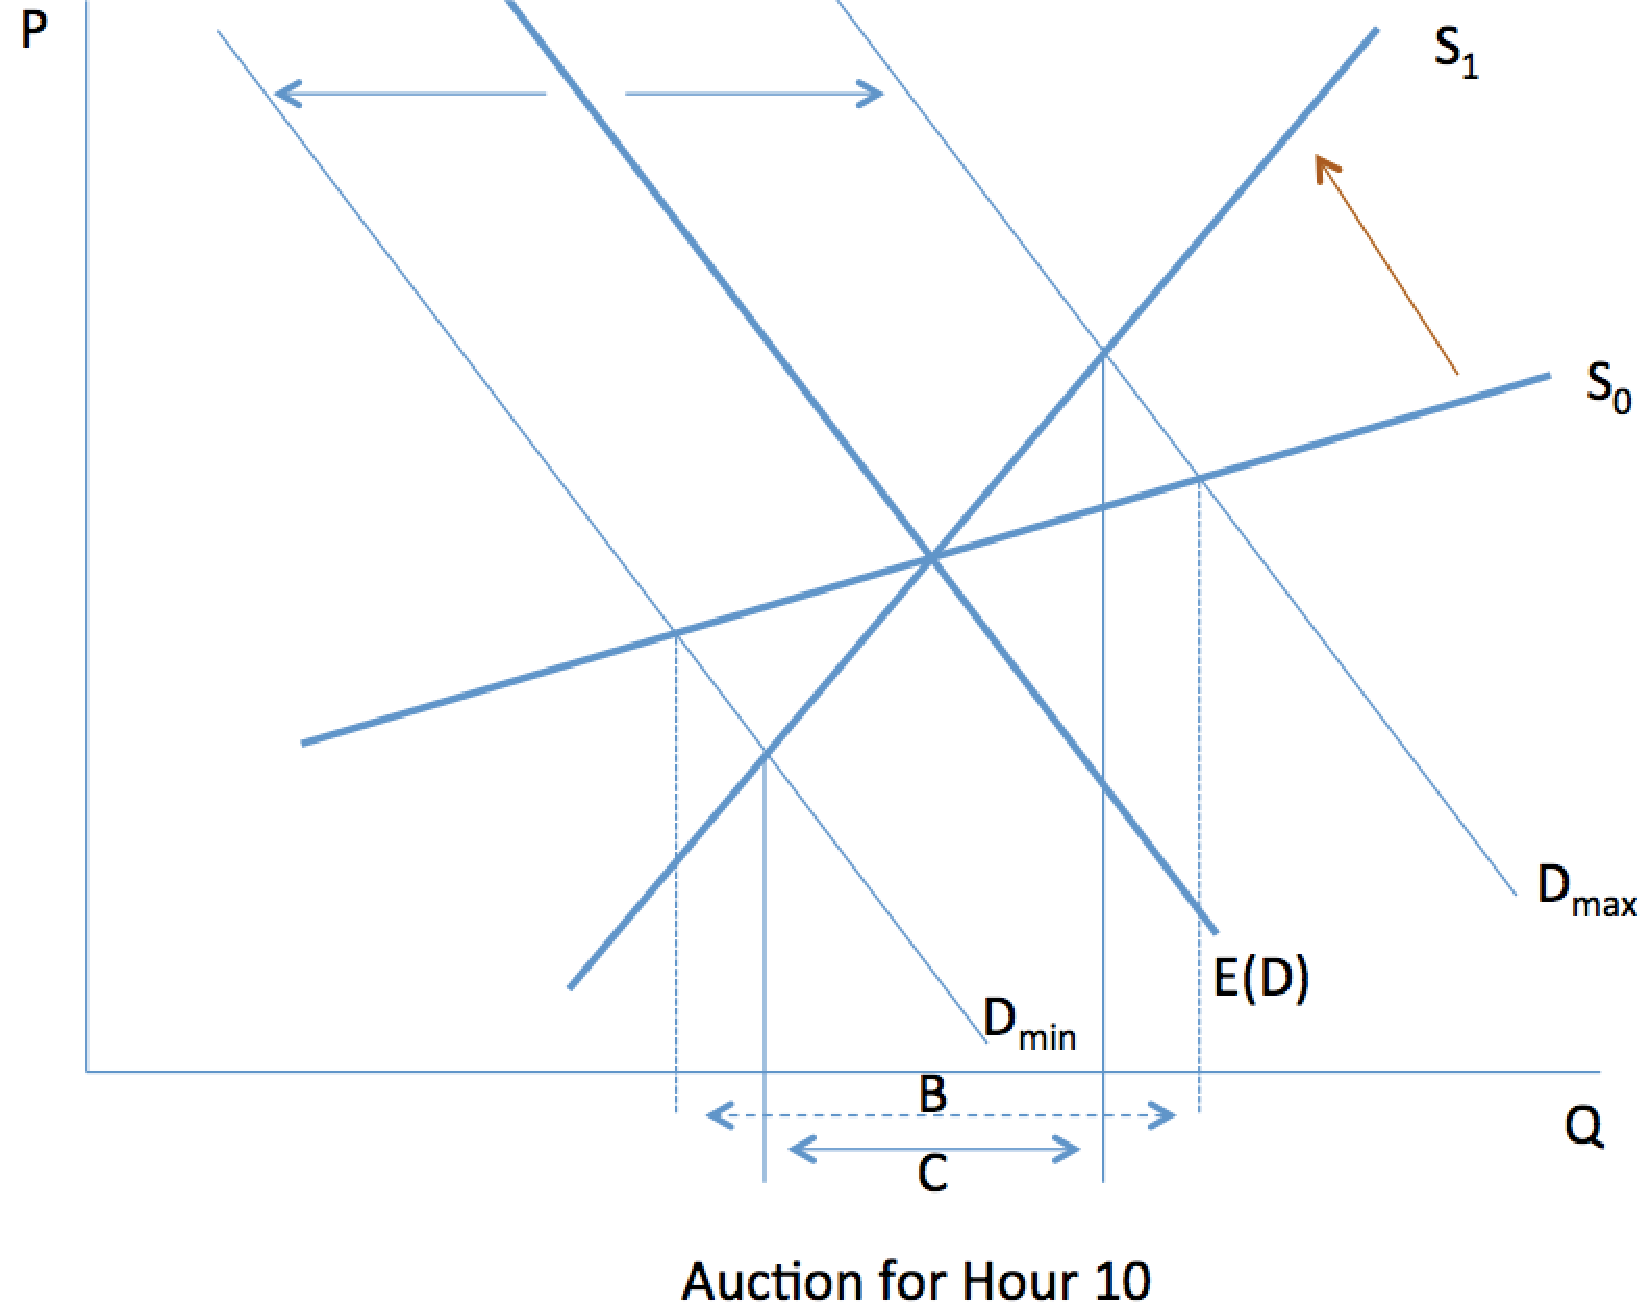
\includegraphics[height=50mm]{figch2/Shot36.pdf} %\hspace{0.03cm} \includegraphics[height=50mm]{predictslope11.pdf}
} \end{center}
\caption{Illustrating the effect of increased uncertainty.}
\label{predictslope}
%{\small Note: }
\end{figure}

The uncertainty in the market is represented %in the model (to move away from model for intuition
 by the width of the envelope of shocks that affect the residual demand function (represented by the arrows on $E(D)$). Thus, in each hour, the residual demand fluctuates between $D_{min}$ and $D_{max}$, where the range between the extremal demands may vary from one hour to the next. 
 
Before submitting a supply function to the market, the supplier estimates the distribution of probabilities of demand shocks that he will face.  %The price elasticity of the supply function is given by the slope of the supply function. 
In hour 9, the supplier is able to rather precisely predict the realisation of the demand function in the auction, i.e. it realises within a tight confidence interval. In hour 10, however, uncertainty in predicting the outcome of the demand realisation has grown strongly as represented by the much wider confidence interval on the demand realisation. 

Given a fixed supply bid function $S_0$, the possible range of quantities to be produced by the supplier when going from hour 9 to hour 10 has increased due to the increase in the size of the uncertainty (interval on the Q-axis has grown from length $A$ for hour 9 to the dotted length $B$ in hour 10).

Now, we assume that the supplier faces dynamic costs, i.e. it is costly for production to vary on top of any traditional marginal cost consideration and the larger the variation, the larger the cost.  Then in the case of a fixed supply bid function ($S_0$ in both auctions), an increase in uncertainty implies an increase in expected dynamic costs. 

The supplier's reaction to increased uncertainty is therefore to bid a steeper supply function $S_1$ in order to trade-off static optimality and dynamic effects. As a consequence, the range of volumes produced in equilibrium is reduced (the firm produces in the range $C$ instead of $B$). When seen over time, these considerations lead to a smoother production as compared to a constant supply curve: demand shocks are absorbed through a higher price volatility and a lower production volatility. %In other words, by introducing dynamic cost considerations, volatility in prices has become comparatively cheaper than volatility in production. 


If cautious behaviour under high uncertainty is true for all firms on the market and each firm has the same expectation of the probability distribution of the uncertainty, then the reaction of bidding a more price inelastic supply function to increased uncertainty should be observable on the aggregated supply function. 

We emphasize that this prediction relies on linear demand and supply functions and does not incorporate capacity constraint considerations (both upper and lower bounds on the production volume of plants), which are also important on the market.  Furthermore, we have outlined our prediction using a discrete time-setting. 
The continuous version of this analysis on dynamic costs is explored in detail by \cite{bergesmartimort2014}. 
%Finally, we consider that the number of bidders stays constant across auctions. Holmberg 2004 shows that the slope of the unique symmetric equilibrium supply function falls with the number of 
% The full blown model solves the problem in the case of a symetric oligopoly of suppliers facing uncertain demand and subject to dynamic costs of production. The essence of the model is for a supplier $i$ to maximise its expected profit: 
%
%\begin{equation}
%\displaystyle{\max_{S_i(p)}}~\mathbb{E}\left[\int_{0}^{T} \left(p(\theta(t))S_i(p(\theta(t))) -C\left(S_i(p(\theta(t))),\frac{dS_i(p(\theta(t)))}{dt} \right)\right)dt\right]
%\end{equation} 
%
%with $S_i(p)$ the supply schedule as a function of the price $p$, $f(\theta)$ the distribution of demand shocks $\theta$, $C(\cdot)$ the cost function depending on the level of production and its variation, $t$ the time, and $T$ the time period over which the flow of profits is maximised. This formula is only presented to give the gist of what is done, the formal maximisation program is different\footnote{This comes from the fact that one of the difficulties lies in the representation of the dynamic costs: the key ingredient in such a model is uncertainty, however, the most natural way to represent dynamic costs is by taking the time derivative of the production. Taking the derivative of a stochastic process is not possible, which is why the program has to be written in a different way. This is a technicality that is developed in much detail in the paper.}.   
%
%This model is solved analytically in the case of linear demand functions and symmetric oligopoly. The main result is that supply functions are linear too, and that their slope evolves with the time derivative of the amount of demand uncertainty. This effect is mainly driven by the use of a time continuous model, which allows to derive analytical results, but which implies myopic solutions: only local dynamic effects (the time derivative of the amount of demand uncertainty) can be derived. The authors believe that this result is a consequence of the continuous formulation of the model, we therefore focus empirically on the impact of the level of uncertainty on the strategies of the suppliers.

The present paper tests this mechanism empirically and understands an increase in the slope of aggregate supply bid functions due to an increased level of uncertainty as evidence that firms minimise dynamic costs across auctions. %\footnote{In a companion paper ***REF, the authors explore the effect of the dynamics of the uncertainty, as opposed to the level of uncertainty investigated in this paper, on the bidding behaviour of electricity supplying firms.}.


%
%This narrative allows for two distinct mathematical interpretations. On the one hand, the absolute level of uncertainty could account for steeper supply schedules. On the other hand, one could think that it is the variation in uncertainty, and not uncertainty itself, that drives the dynamic bidding behaviour. 
%
%The first interpretation is straightforward from the previous paragraphs. The second one comes from a more detailed analysis of the dynamics of demand shocks. More precisely, when modelling shocks it is possible to obtain a situation where the level itself of uncertainty is not the driving force but the variation of the uncertainty is. This distinction can arise when a the level of demand is close to its expected maximum or minimum value. Close to the boundaries, it is expected to stay there longer than if it is close to its expected value. One can think of this as a producer forming his anticipation of demand based on different demand scenarios. 
%
%There can be many different situations leading to an average demand, but for demand to be close to its maximum or minimum anticipated value, a lot of events must realise in a specific way. Therefore, when close to a boundary, there is not much uncertainty as to which scenario lead to such a situation, whereas multiple scenarios can lead to an average demand value. The level effects of uncertainty, i.e. when close to a boundary there is less potential variation in demand than when close to its expected value, may cancel out, leaving the dynamics of the uncertainty as the only driver for bid shifting of suppliers : when uncertainty increases these effects become unbalanced and optimal bids change.


%These effects, i.e when close to a boundary there is less potential variation in demand than when close to its expected value, can balance out and leave only a pure dynamic effect, that is that the variation in uncertainty drives the dynamics of the optimal bid submitted by producers: when uncertainty increases these effects become unbalanced and optimal bids change. 
%
%Berg\`es and Martimort (in prep) develop a full mathematical analysis of the dynamics of supply function equilibria under uncertainty when production is subject to dynamic costs, which points towards the possibility for the second more involved and less intuitive effect to exist. This paper tests empirically both mechanisms and understands an increase in the slope of aggregate supply bid functions due to increased uncertainty as evidence that firms minimise dynamic costs across auctions.

%If there is low uncertainty on both low and high frequency volatility over time, the supplier can reasonably well anticipate the dynamic costs between production volumes. If now there is high uncertainty on high frequency volatility (noise) and low uncertainty on the trend, it means that the specific trajectory of demand is quite uncertain but it might not change much statistically speaking from a well anticipated trajectory. On the contrary, what can be quite informative is the variation in uncertainty. If the uncertainty increases sharply, it means that we know that there might be large shocks to the demand, which is not the same as having a low amount of information about an otherwise typical demand trajectory during the day. 

%In other words, constant high uncertainty can point towards daily shocks, i.e. the anticipation of the heating required for the day was off for every hour by the same amount, whereas varying uncertainty can point towards knowledge of local shocks than can lead to high dynamic costs. This is why variation in uncertainty could be the actual driving force behind changes in supply curves from hour to hour. The paper by \cite{bergesmartimort2014} predicts the latter relationship. This paper tests empirically both mechanisms and understands an increase in the slope of aggregate supply bid functions due to increased uncertainty as evidence that firms minimise dynamic costs across auctions.

%
%*********
%
%Alternative idea of explanation: 
%
%Costly variation in the predictability of demand shock is due to to coordination failures in the market. When uncertainty increases sharply, many firms in the industry aim to adjust their bidding behaviour. Expectation differences (does not work with symmetric players) lead to exacerbation of natural uncertainty and thus increase dynamic costs. 
%Private information in bidding distorts the adjustment bidding behaviour of firms and can exacerbate over/undershooting of aggregate bid expectation when adjusting to new uncertainty environment. 
%
%*********



\section{The EPEX spot market}
\label{epexall}
\subsection{General background}
\label{epexbackground}
The EPEX Spot market is an auction market, which allows firms to trade electricity 12-36h ahead of delivery. It covers France, Germany with Austria and Switzerland. The volume traded on Epex Spot represents $12\%$, $40\%$ and $30\%$ of the total electricity consumption in these countries respectively in 2013 \cite{epexwebsite1}.

The EPEX Spot market has considerably gained in importance over time and the daily trading volume has almost quadrupled since $2005$, whereas the total electricity consumption has essentially remained constant. The graph in figure \ref{volconsfr} shows these trends very clearly. Furthermore, it shows the significant volatility of the market trading volume (as indicated by the width 
%\footnote{Figure \ref{rollsdvolconsfr} in the appendix shows the evolution of the standard error on which the confidence interval in figure \ref{volconsfr} is based.} 
of the grey-shaded confidence interval).  
\begin{figure}[!ht]
\begin{center} \makebox[\textwidth]{
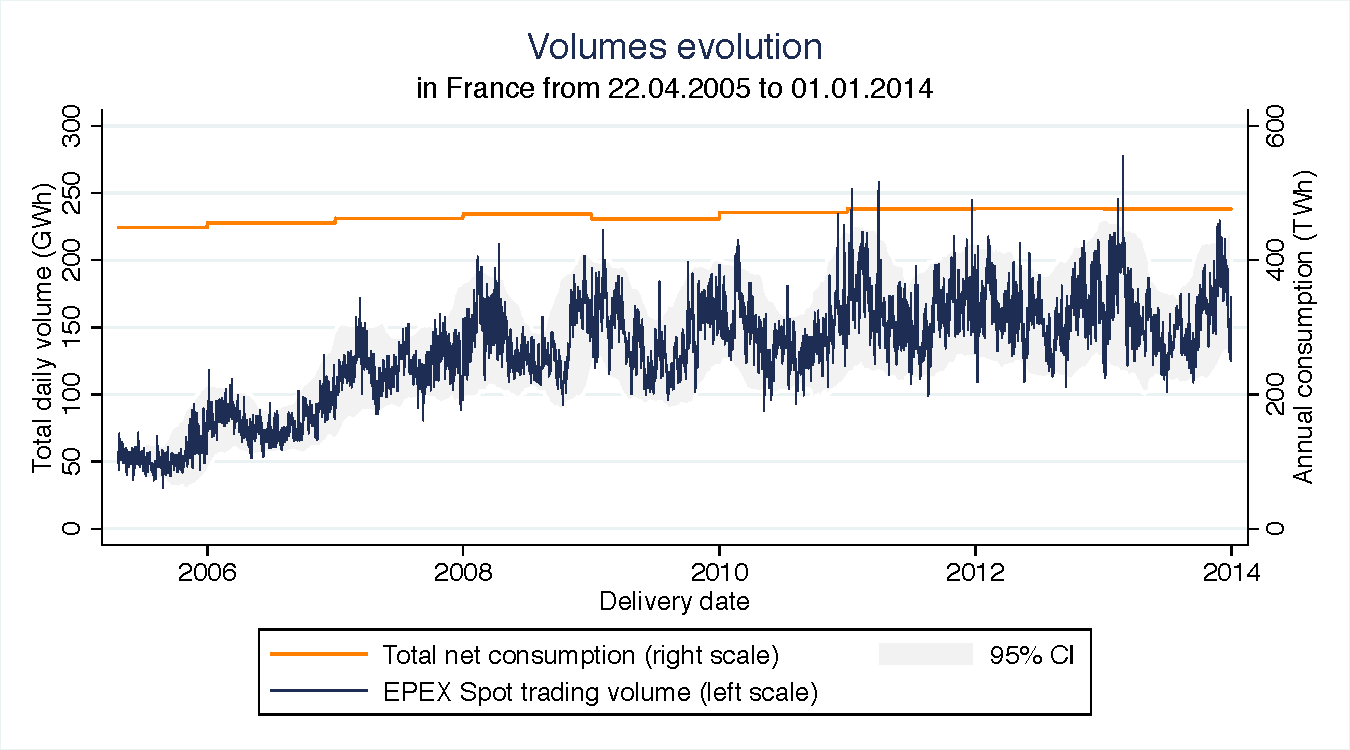
\includegraphics[height=74mm]{figch2/volplusconso3.pdf} 
} \end{center}
\caption{Traded volume plotted against total annual consumption}
\label{volconsfr}
% graph updated on 24.11.2014
{\small Note: Total consumption is netted of the electricity withdrawal at the level of the production unit. The 95\% confidence interval is based on a 150-days moving window and assumes that volumes are normally distributed in the time window. GWh and TWh stand for giga and terawatt hours, respectively.}
\end{figure}


%EPEX SPOT provides a liquidity outlet for the producers, the suppliers and the transmission system operators, as well as for the industrial consumers, to fulfil their sales or their purchases in short term power \cite{epexwebsite1}.
On the EPEX Spot market, the participants submit supply or demand bid functions to be able to meet their next day's supply commitment. 
This market is important, because it allows the firms to adjust their  portfolio to the upcoming demand. The market matches business to business trades, where producers (the suppliers and transmission system operators) and industrial consumers may participate.

%the following firms may participate in the market: All primary (e.g. EDF) and secondary (e.g. Poweo\footnote{Power does not own nuclear electricity generating units, but buys this energy in bulk from primary producers, e.g. in the wholesale virtual power plant auctions, where EDF sells virtual nuclear capacity to rival firms who are not allowed by the government to run nuclear plants independently.}) electricity supplying firms, intermediate electricity resellers (e.g. XXXXX to complete) and large-scale electricity consumers (e.g. aluminium plants). The minimum barrier to entry is XXXXXX. %to complete

The EPEX Spot market settles in a three-pronged market that firms use to achieve their desired power position: The long-term bilateral contracting market, the day-ahead market and the intra-day market. Energy cannot be stored, thus an precise power position must be achieved at each point in time. Firms thus face a trade-off between cheap up-front sourcing and costly uncertainty. The closer the market gets to the delivery of its power, the less uncertainty does the firm face in determining its power requirements (pushing firms to wait until the last minute to fill their energy position). However, the imperfect flexibility of the electricity production landscape cannot satisfy the whole demand short-term at a reasonable price, hence firms must anticipate their requirements in order to obtain cheaper power. Consequently, these three markets complement each other to allow firms to gather a power position at a reasonable price. 


	%%%%%%%%%%%%%%%%%%%%%%%%%%%%%%%%%%%%%%%%%%%%%%
	% Brief account of auction mechanism 
	%%%%%%%%%%%%%%%%%%%%%%%%%%%%%%%%%%%%%%%%%%%%%%
\subsection{Auction rules and mechanism}
\label{epexrules}
The EPEX Spot auction occurs daily, all year-round, and proceeds as follows: the order book closes every day at noon for contracts of the following day, results are published two hours later. Bids may be submitted 24/7 from 45 days prior until the closing of the books. 

Tradable contracts exist for each hour of the day and firms submit an individual bid function for each of these hours, i.e. a separate, simultaneous auction is run for all hours of the following day and trading is specific for each of these hourly tranches.  

The bid submission must be a supply function (or a demand function depending on the position of the firm) with at least 2 and at most 256 price/quantity combinations for single contract orders. The final bid function, thus, consists of the explicitly submitted points and all linearly interpolated points between them. The bid curves must be monotonically increasing for a supply function and vice versa for a demand function. Orders are transmitted via an online IT-platform and a redundant confirmation process aims to avoid erroneous bids. Bids are anonymous and the final electricity distribution is done via the French distribution network controlled by RTE EDF Transport SA. 

%Furthermore, the French day-ahead market is coupled with the intraday and forward markets % HOW????? TO explain in a footnote
%as well as the day-ahead markets of some of its European neighbours, e.g. the German market\footnote{Formally known under \textit{Leipziger Stromb\"{o}rse}.}% TO confirm 
%. In the case of national market coupling, the effectiveness of the coupling is subject to the physical laws underlying electricity transfer (e.g. laws of XXXXX) %la loi qui rends le transfer d'electricity hyper complique a calculer dans un reseau.. :)

	%%%%%%%%%%%%%%%%%%%%%%%%%%%%%%%%%%%%%%%%%%%%%%
	% Bidding
	%%%%%%%%%%%%%%%%%%%%%%%%%%%%%%%%%%%%%%%%%%%%%%
Prices are specified in \euro{}/MWh with two decimal digits and must range from -3000\euro{}/MWh to +3000\euro{}/MWh. Quantities are specified in whole MWh. In addition to single contract orders for an individual hour, bidders may submit block orders. 
These are combined single contract orders with a minimum of two consecutive hours. The vital difference with multiple single contract orders is the "All-or-None" condition, namely that the executions of the individual contract orders forming the block are dependent on one another. That is for a block order covering hours 17 to 20, the quantity demanded for the hour 17 is only awarded if the corresponding quantity is also awarded for the hours 18, 19 and 20. Each registered bidder account is limited to a maximum of 40 block orders per delivery day, each of which is limited in volume to 400 MWh (approx. equal to $0.25\%$ of total daily volume traded on EPEX Spot). 

	%%%%%%%%%%%%%%%%%%%%%%%%%%%%%%%%%%%%%%%%%%%%%%
	% Price determination
	%%%%%%%%%%%%%%%%%%%%%%%%%%%%%%%%%%%%%%%%%%%%%%
The price-quantity determining mechanism is a uniform price, multi-unit auction mechanism: the summed demand and supply curves are computed and the intersection of these gives the equilibrium price and quantity pair. The market clearing mechanism takes into account single and block orders simultaneously and hence solves the corresponding programme by an algorithm of full enumeration of possible solutions, where each partial solution is verified to provide real, compatible prices. %When no explicit bid point exists at the point of intersection, the algorithm linearly interpolates between the closest points.  - already in function definition included
The mechanism works under a time limit. In the case of a curtailment, i.e. a disequilibrium with disproportionate prices due to unmatched supply and demand or an abnormal price for a specific hourly contract, the system proceeds to a second price fixing. 

	%%%%%%%%%%%%%%%%%%%%%%%%%%%%%%%%%%%%%%%%%%%%%%
	% Information distribution in the market, what players know when bidding
	%%%%%%%%%%%%%%%%%%%%%%%%%%%%%%%%%%%%%%%%%%%%%%
Of particular interest is the clear distribution of information. Ex-ante bidding, firms in the market know the identities of the rival bidders they face (but neither their individual bid functions nor their results in past auctions), the history of aggregated equilibrium prices and quantities up to that day, their clients' past demand realisations and their individual long term contracting position. Upon the clearing of the market, the aggregated supply and demand bid functions, equilibrium quantity and the equilibrium price become common knowledge. Each bidding account is informed of the contracts it has been awarded, i.e. the individual quantities to be sold and bought through the system.


\section{Our data explained}

%%%%%%%%%%%%%%%%%%%%%%%%%%%%%%%%%%%%%%%%%%%%%%%
%%%%%%%%%%%%%%%%%%%%%%%%%%%%%%%%%%%%%%%%%%%%%%%
%----*** REMOVE AND PUT IN OTHER CHAPTER
\label{pschapter}
%%%%%%%%%%%%%%%%%%%%%%%%%%%%%%%%%%%%%%%%%%%%%%%
%%%%%%%%%%%%%%%%%%%%%%%%%%%%%%%%%%%%%%%%%%%%%%%

\label{datasection}
\subsection*{Auction market data}
We have data from the French EPEX Spot market for the period 01.01.2011 to 30.06.2013. This is the latest period, where no significant changes in the auction rules have occurred and where data for all variables can be observed. 

We observe the full aggregate bid functions for the day-ahead auctions of each hourly contract for both supply and demand. 
We understand the dataset as a cross-section rather than a time-series\footnote{This is supported by the graph in figure \ref{volconsfr}, which shows a flat total consumption and average trading volume on EPEX Spot since 01.01.2011.} and focus on weekday trading contracts only. 
This sums up to about 31 500 observations\footnote{31 500 observations $\approx 2.5$ years of hourly ($*365 *24$) demand and supply ($*2$) functions for weekday trading ($*5/7$).}. A single aggregate bid function is the sum of the individual bid functions, which are not available. %for competition reasons. 
We also observe the equilibrium price and quantity for each auction.

Moreover, we observe the block bidding results at the equilibrium solution only. We ignore the blocked aspects and treat subsequent auctions as independent from one another.
	
	%%%%%%%%%%%%%%%%%%%%%%%%%%%%%%%%%%%%%%%%%%%%%%
	% Graphical example of the data we have. 
	%%%%%%%%%%%%%%%%%%%%%%%%%%%%%%%%%%%%%%%%%%%%%%
The two graphs in figure \ref{examplebidfunc} show the aggregate supply and demand bid functions for the same hour of the same day. For a glimpse at the variation of bid functions over time, see figure \ref{graphmultifunc}. The table \ref{overallsummary} sheds some light on the raw data. For further details as well as the plotted distribution of realised market equilibria, refer to appendix \ref{statdes1}. 

Finally, we reuse the data output from chapter \ref{pschapter}. Specifically, we reuse the specific points extracted from the aggregate demand and supply bid functions, which are comparable across auctions. Why these points are useful for our analysis is explained in the methodology (section \ref{newapproach}).

\begin{figure}[!ht]
\begin{center} 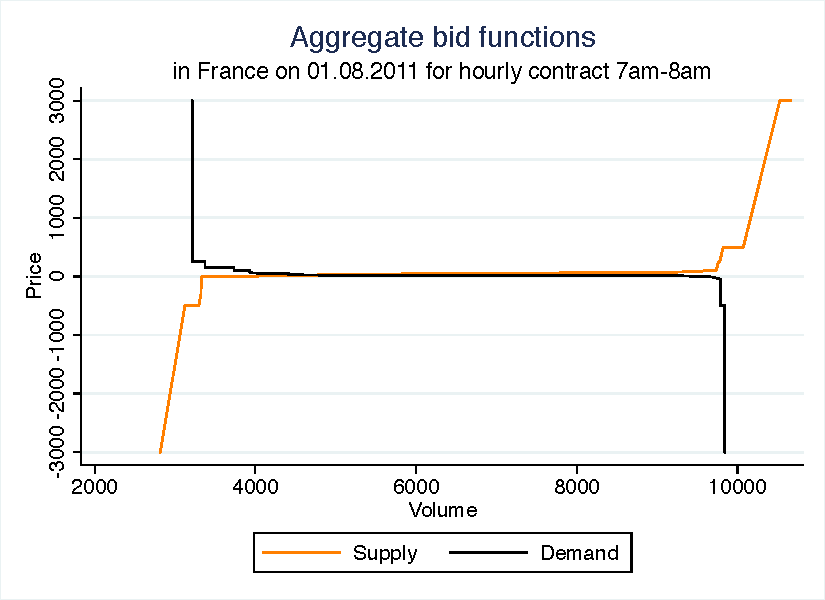
\includegraphics[height=50mm]{figch2/aggbidfuncnozoom.pdf} \hspace{0.05cm}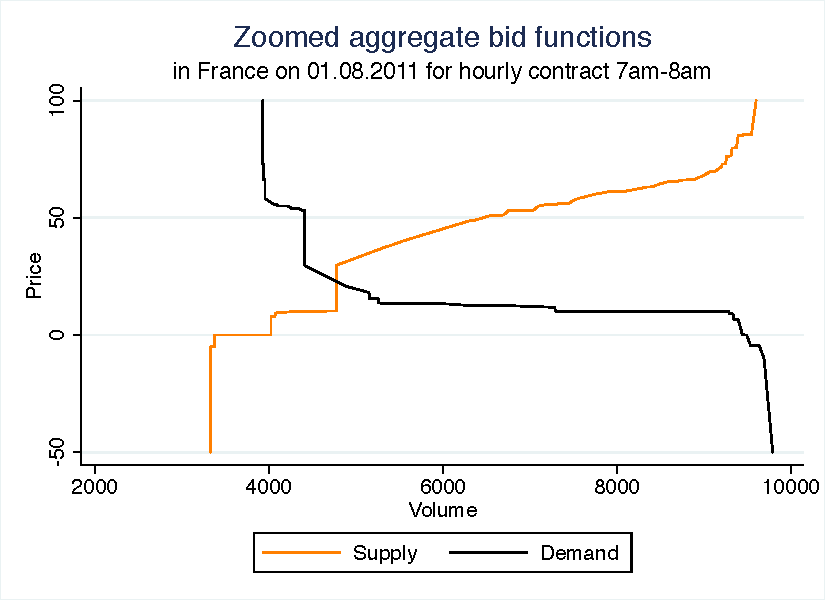
\includegraphics[height=50mm]{figch2/aggbidfuncwithzoom.pdf} \end{center}
\caption{Example aggregate demand and supply bid functions}
\label{examplebidfunc}
{\small Note: The right-hand-side graph is a zoom of the left graph on for the price range  $-50$\EUR{}/MWh  to +100\euro /MWh.}
\end{figure}


\begin{figure}[!ht]
\vspace{0.3cm}
\begin{center}\makebox[\textwidth][c]{
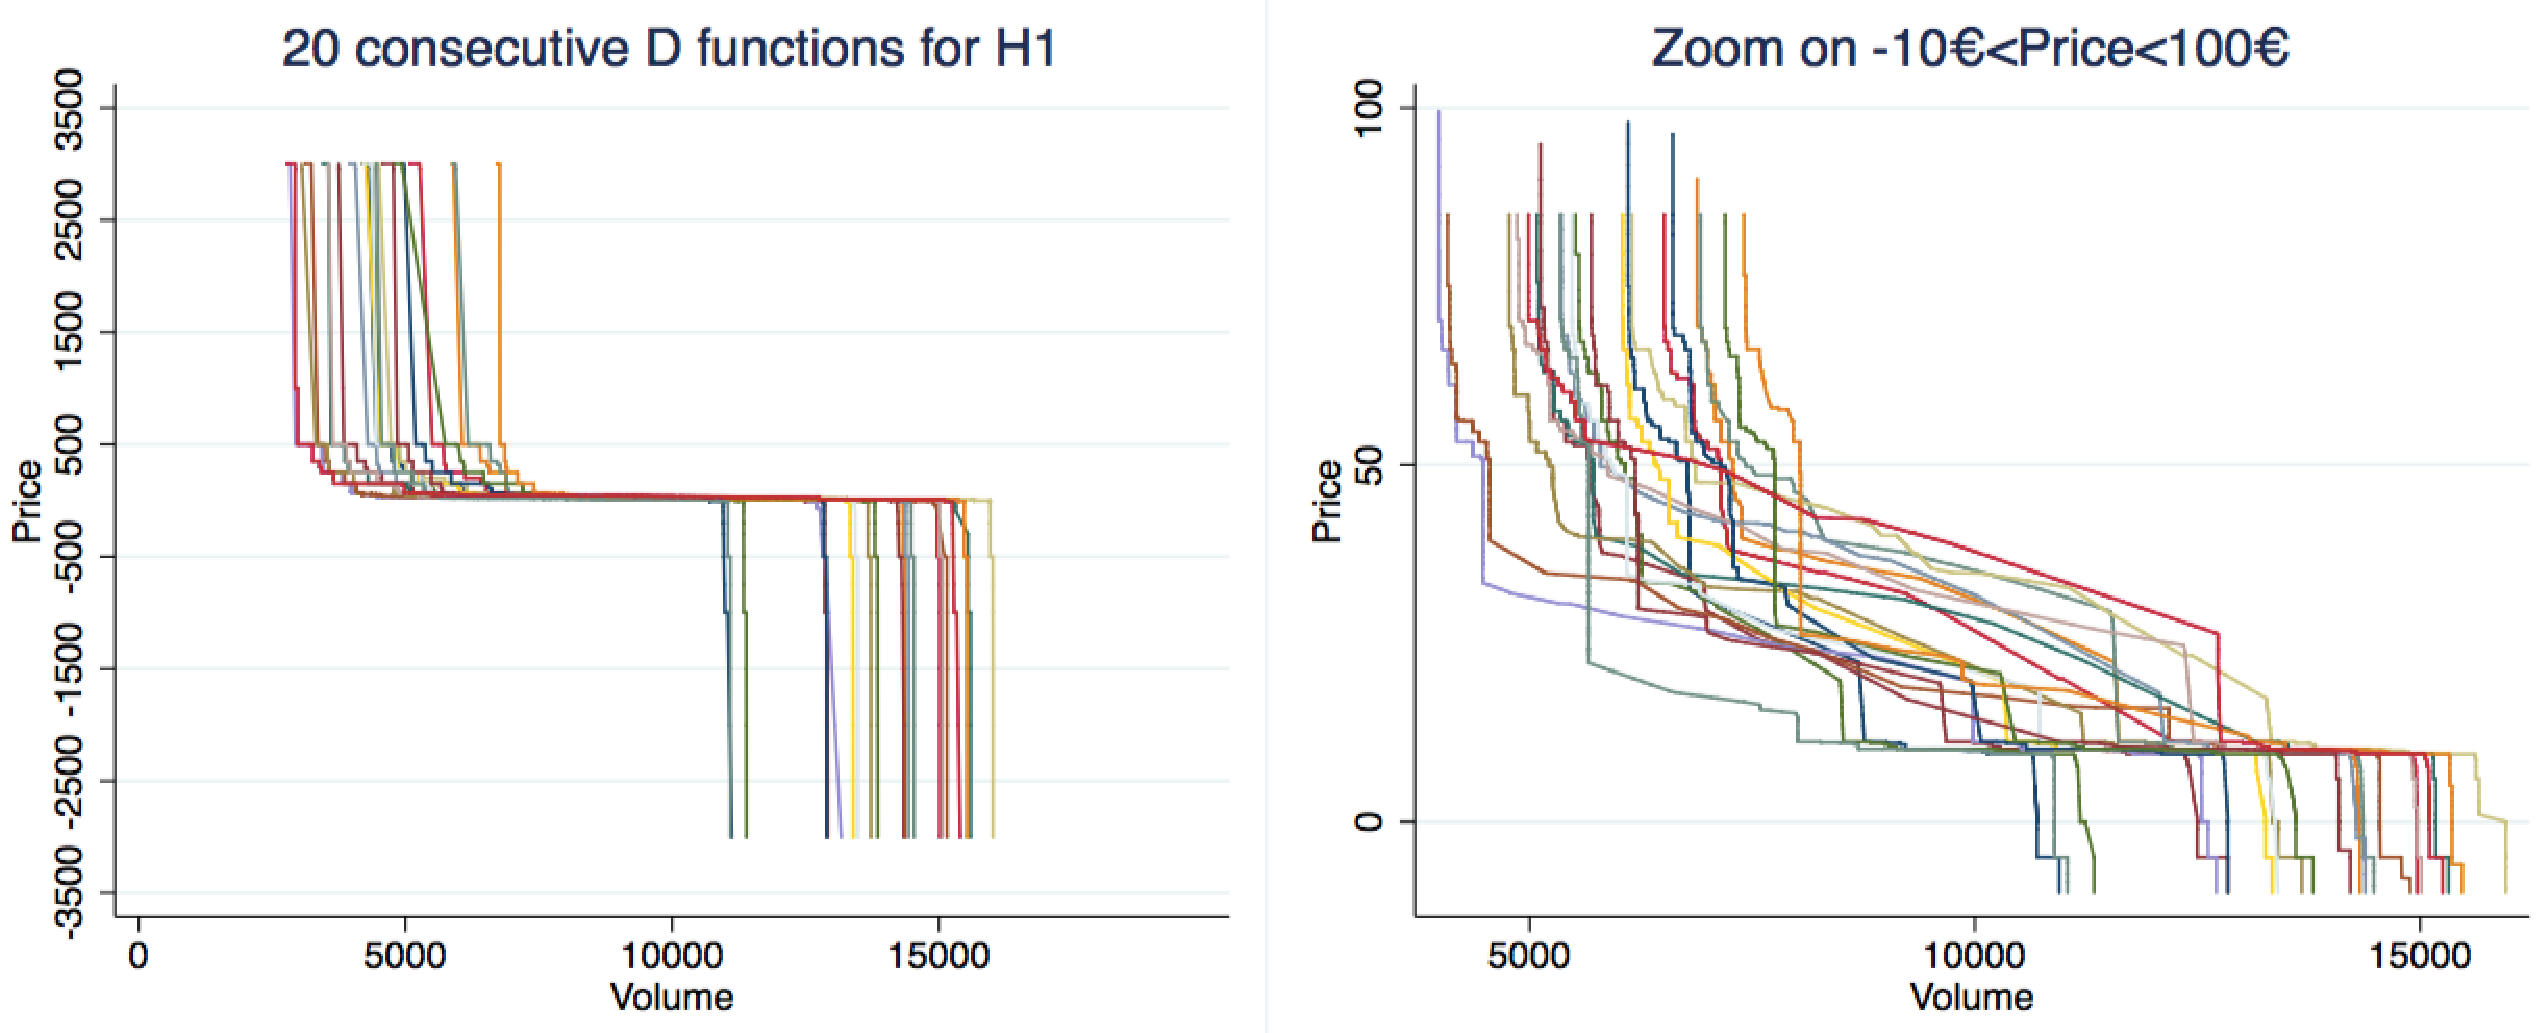
\includegraphics[height=50mm]{figch2/Shot28.pdf}
}\\
\vspace{0.05cm}
\makebox[\textwidth][c]{
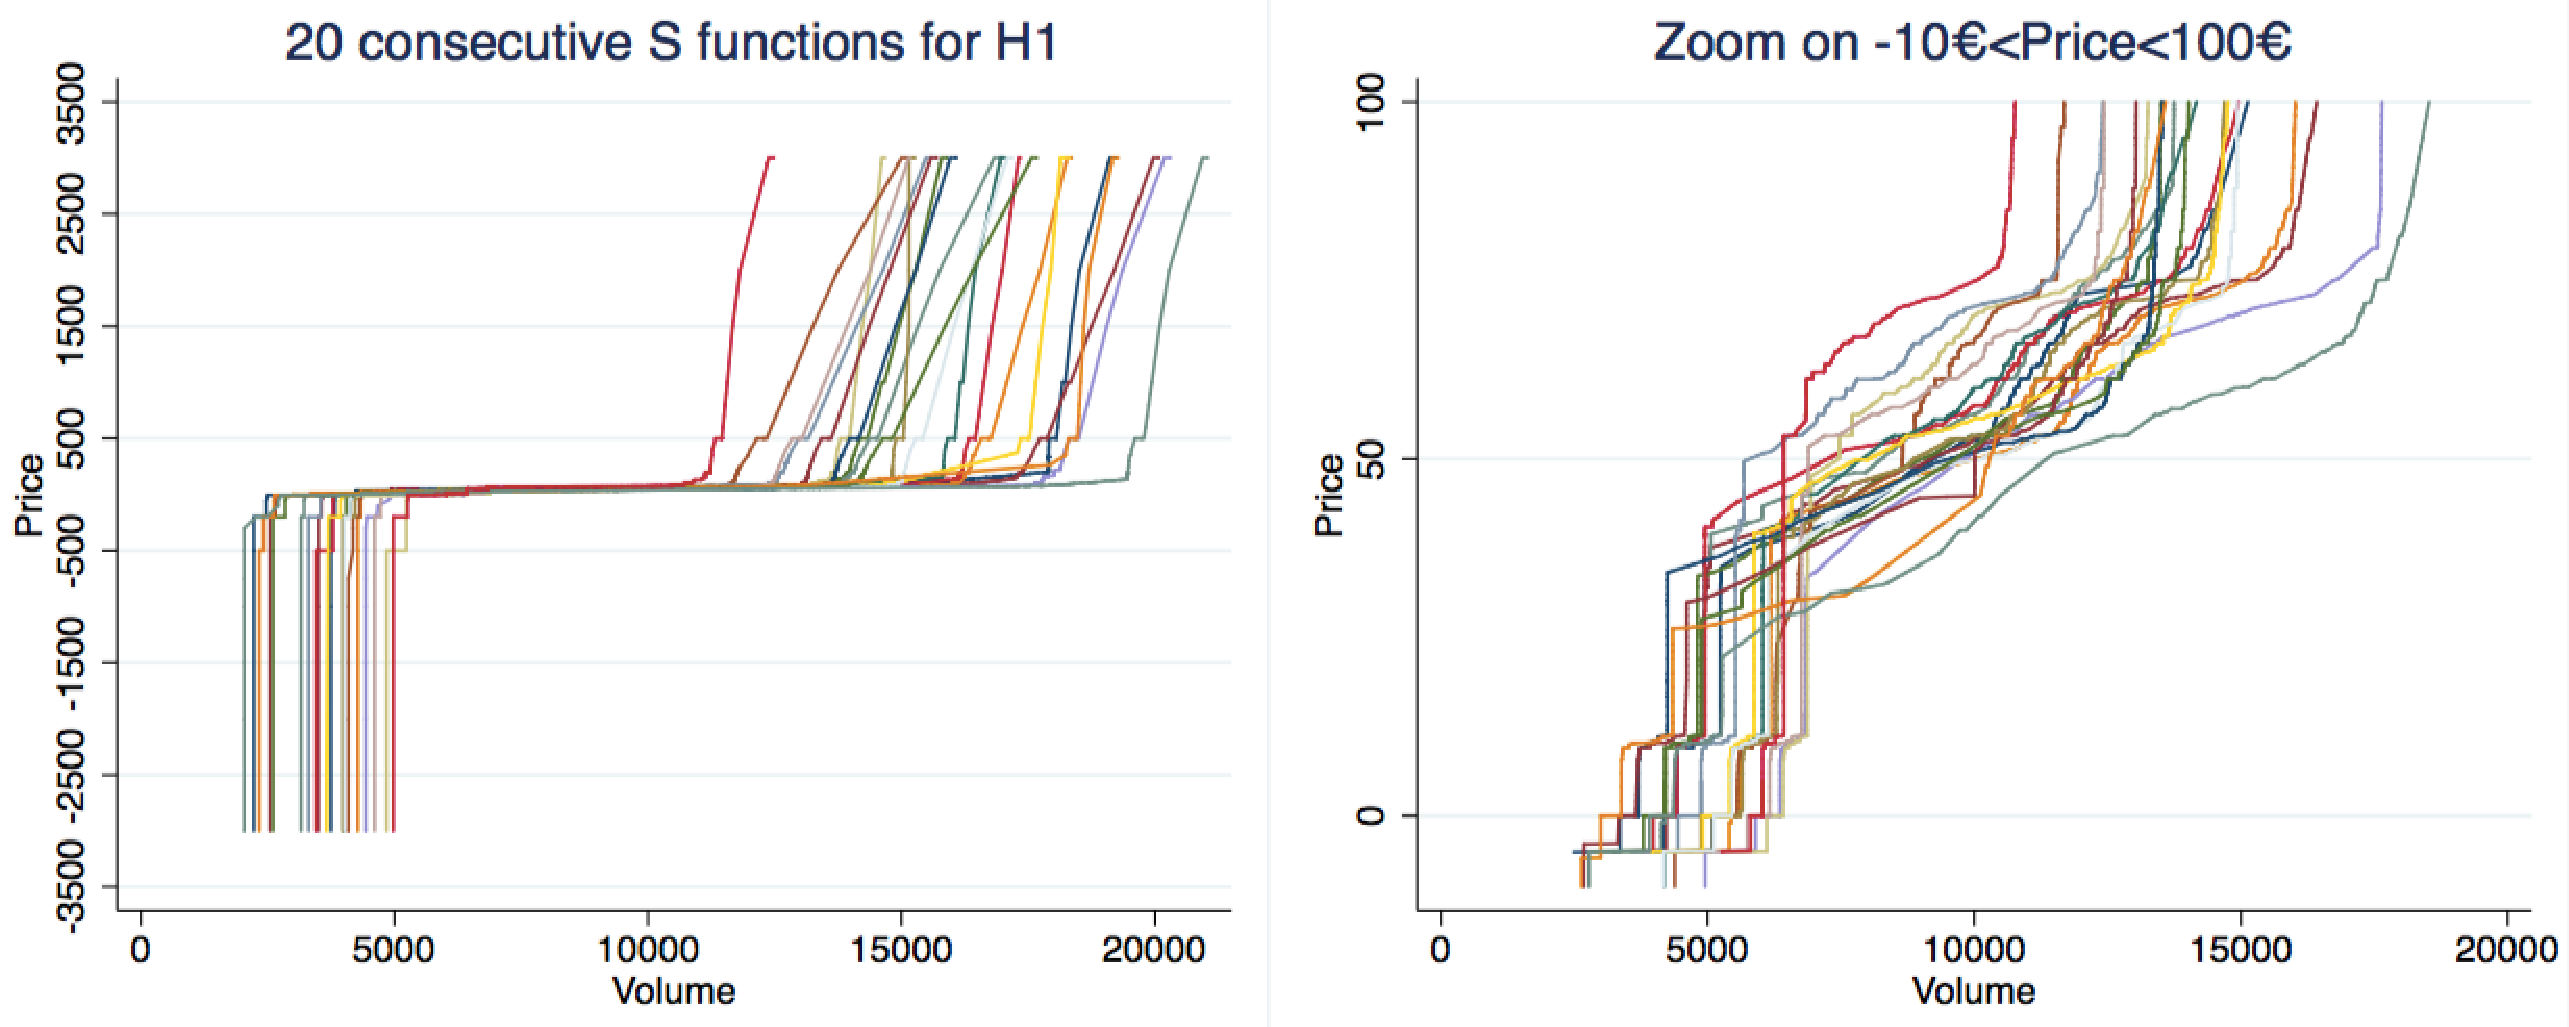
\includegraphics[height=50mm]{figch2/Shot27.pdf}
}
\caption{Aggregate bid functions for 20 consecutive days}
\label{graphmultifunc}
\end{center}
{\small Note: The graph shows 20 consecutive aggregate demand and supply functions for the contracts on hour 1 (between 12am and 1am) for the time period 11/12/2011 to 31/12/2011. The graph on the right is a zoom on the price elastic region of the curves on the left.}
\end{figure}

	%%%%%%%%%%%%%%%%%%%%%%%%%%%%%%%%%%%%%%%%%%%%%%
	% Tabular data to give an example
	% Keep LONGTABLE TO HAVE FOOTNOTES APPEAR. 
	%%%%%%%%%%%%%%%%%%%%%%%%%%%%%%%%%%%%%%%%%%%%%%	
%\setlength{\LTleft}{-20cm plus -1fill}
%\setlength{\LTright}{\LTleft}
%\setlength{\LTpre}{18pt}
%\setlength{\LTpost}{0pt}
%\newgeometry{margin=2cm} 
%\begin{landscape}
%\footnotesize
%\begin{table}[!ht]
%\vspace{-1.4cm}


\begin{center}
% matrix: out1 file: /Users/Orie/Cloud/Google Drive - Account henridb1/Encheres Elec/Article/overallsummary.tex   1 Oct 2014 15:48:56
\begin{center}
\begin{longtable}{lrrrrr}
\toprule
 & Mean  & Median  & Std. Dev  & Min  & Max  \\
\midrule
\endfirsthead
\multicolumn{6}{l}{\emph{... table \thetable{} continued}} \\
  & Mean  & Median  & Std. Dev  & Min  & Max  \\
\midrule
\endhead
\midrule
\multicolumn{6}{r}{\emph{Continued on next page...}}
\endfoot
\endlastfoot
Total daily volume &  161,912 &  159,313 & 25,059 & 99,054 &  277,531 \\  
Average realised daily price\footnote{Average price is volume weighted over the 24 hourly contracts of the delivery day.} &    46.6 &    48.3 &    17.2 &   -39.0 &   381.2 \\  
%Congruence ratio\footnote{It is defined by the ratio of maximum supplied volume to maximum demanded volume. It is based on \cite{armstronggalli2007empirical} and measures liquidity in the market by comparing how similar buyer and seller attitudes to trade are on the market. The authors find that unusually high prices generally occur when this metric exceeds 2.} &     1.11 &     1.07 &     0.32 &     0.45 &     4.51 \\  
Minimum demanded agg. volume\footnote{Minimum and maximum volumes for both demand and supply refer to the aggregate volume bid on the market for a single hour contract at the extremal prices of $+3000$\euro /MWh or $-3000$\euro /MWh.} & 5,030 & 4,968 & 1,467 &   914 & 11301 \\  
Maximum demanded agg. volume & 13,327 & 13,222 & 2,212 & 4,990 & 23,254 \\  
\midrule
Minimum supplied agg. volume & 3,721 & 3,526 & 1,344 &   618 & 10594 \\  
Maximum supplied agg. volume & 14,390 & 14,142 & 3,051 & 6,580 & 35,356 \\  
Bid points per demand function &   543 &   531 &   163 &   115 & 1,253 \\  
Bid points per supply function &   640 &   632 &   143 &   184 & 1,283 \\  
Bidders per auction\footnote{Due to the anonymity of the auction procedure, it is unknown which bidders submitted bids. Consequently, it cannot be deduced how many bid steps a typical bidder submits. Number of registered bidders for the French EPEX Spot market as of 01.10.2014.} &   - &    - &   - &   1 & 101 \\
\bottomrule
\caption{\label{overallsummary} Some descriptive statistics}
\end{longtable} 
\end{center}
%\caption{\label{overallsummary} ***}
\end{center}
%\emph{Note}:
%\end{table}
%\end{landscape}
%\restoregeometry


		%%%%%%%%%%%
		% can include more info on number on functions observed and give 
		% tabular stata at 3 year level for weekday only. 
		% say we focus on weekdays, not distinction between mo and tues
		%%%%%%%%%%
\subsection*{Exogenous factors}
	%%%%%%%%%%%%%%%%%%%%%%%%%%%%%%%%%%%%%%%%%%%%%%
	% Meteo data
	%%%%%%%%%%%%%%%%%%%%%%%%%%%%%%%%%%%%%%%%%%%%%%

Regarding weather statistics, we have hourly previsions for temperature, wind and cloudiness from the GFS (Global Forecast System) as well as hourly observations for these quantities and luminosity from M\'{e}t\'{e}oFrance
. The previsions from the GFS are in the form of weather maps that are outputted from simulations that run one-day ahead at 6 am. This is the weather information that market participants have access to when bidding on EPEX Spot\footnote{The next weather simulation run takes place at 12 noon, and is therefore not being used by the bidders on the EPEX day-ahead market, as the deadline for submitting bids is precisely 12 noon.}. The weather observations are in the form of tables for specific weather stations (between 100 and 200 depending on the specific parameter of interest).

Moreover, we have the location of the total installed capacity per generation type (i.e. wind turbines, solar panels, etc.) at the level of the postcode, that is roughly a 3km precision. We obtain this data from the SOeS, a branch of the French government producing data on environmental issues at large. 

Population data and data on the level of the domestic production from the manufacturing industry is obtained in monthly steps from the French National Institute of Statistics and Economic Studies (INSEE). From the same source, we obtain the spot prices for petrol and natural gas as well as the import prices at the border for coal, which we use as a proxy for the domestic prices. 
Prices for the European CO2 emission certificates are taken from the Portuguese secondary market (SENDECO$_2$) for European Unit Allowances (EUA)\footnote{Each unit EUA permit allows one tonne of CO2 emissions.}.

As a very coarse proxy for generation from hydro power plants, we have the total weekly stock of water in domestic dams (in the form of the summed height of all dam water levels in France) from RTE the grid operator.









\section{The economic model}

\section{The political model}

\section{Property rights institutions}

\section{Conclusion}


\begin{subappendices}
\section*{Appendix}
\addcontentsline{toc}{chapter}{Appendix}
\numberwithin{figure}{section}
\numberwithin{equation}{section}

\section{Feasible investments (proof of Prop. n°)}


\end{subappendices}